The main goal is to assess how well can the customer path be approximated given the CDR events they generate.
We examine how accurately we can estimate a customer's route given
\begin{itemize}
    \item sequence of mobile network events generated by them (CDR data),
    \item cell tower data (cell map) to obtain location information for the connected cells.
\end{itemize}

For validation we use the trajectory of GPS locations, which are considered as ground truth.

More specifically, we compare ground truth GPS trajectories to trajectories of CDR events for the same time window in a distributed fashion as shown in Figure \ref{fig:problem}. 
\begin{figure}[h]
    \centering
    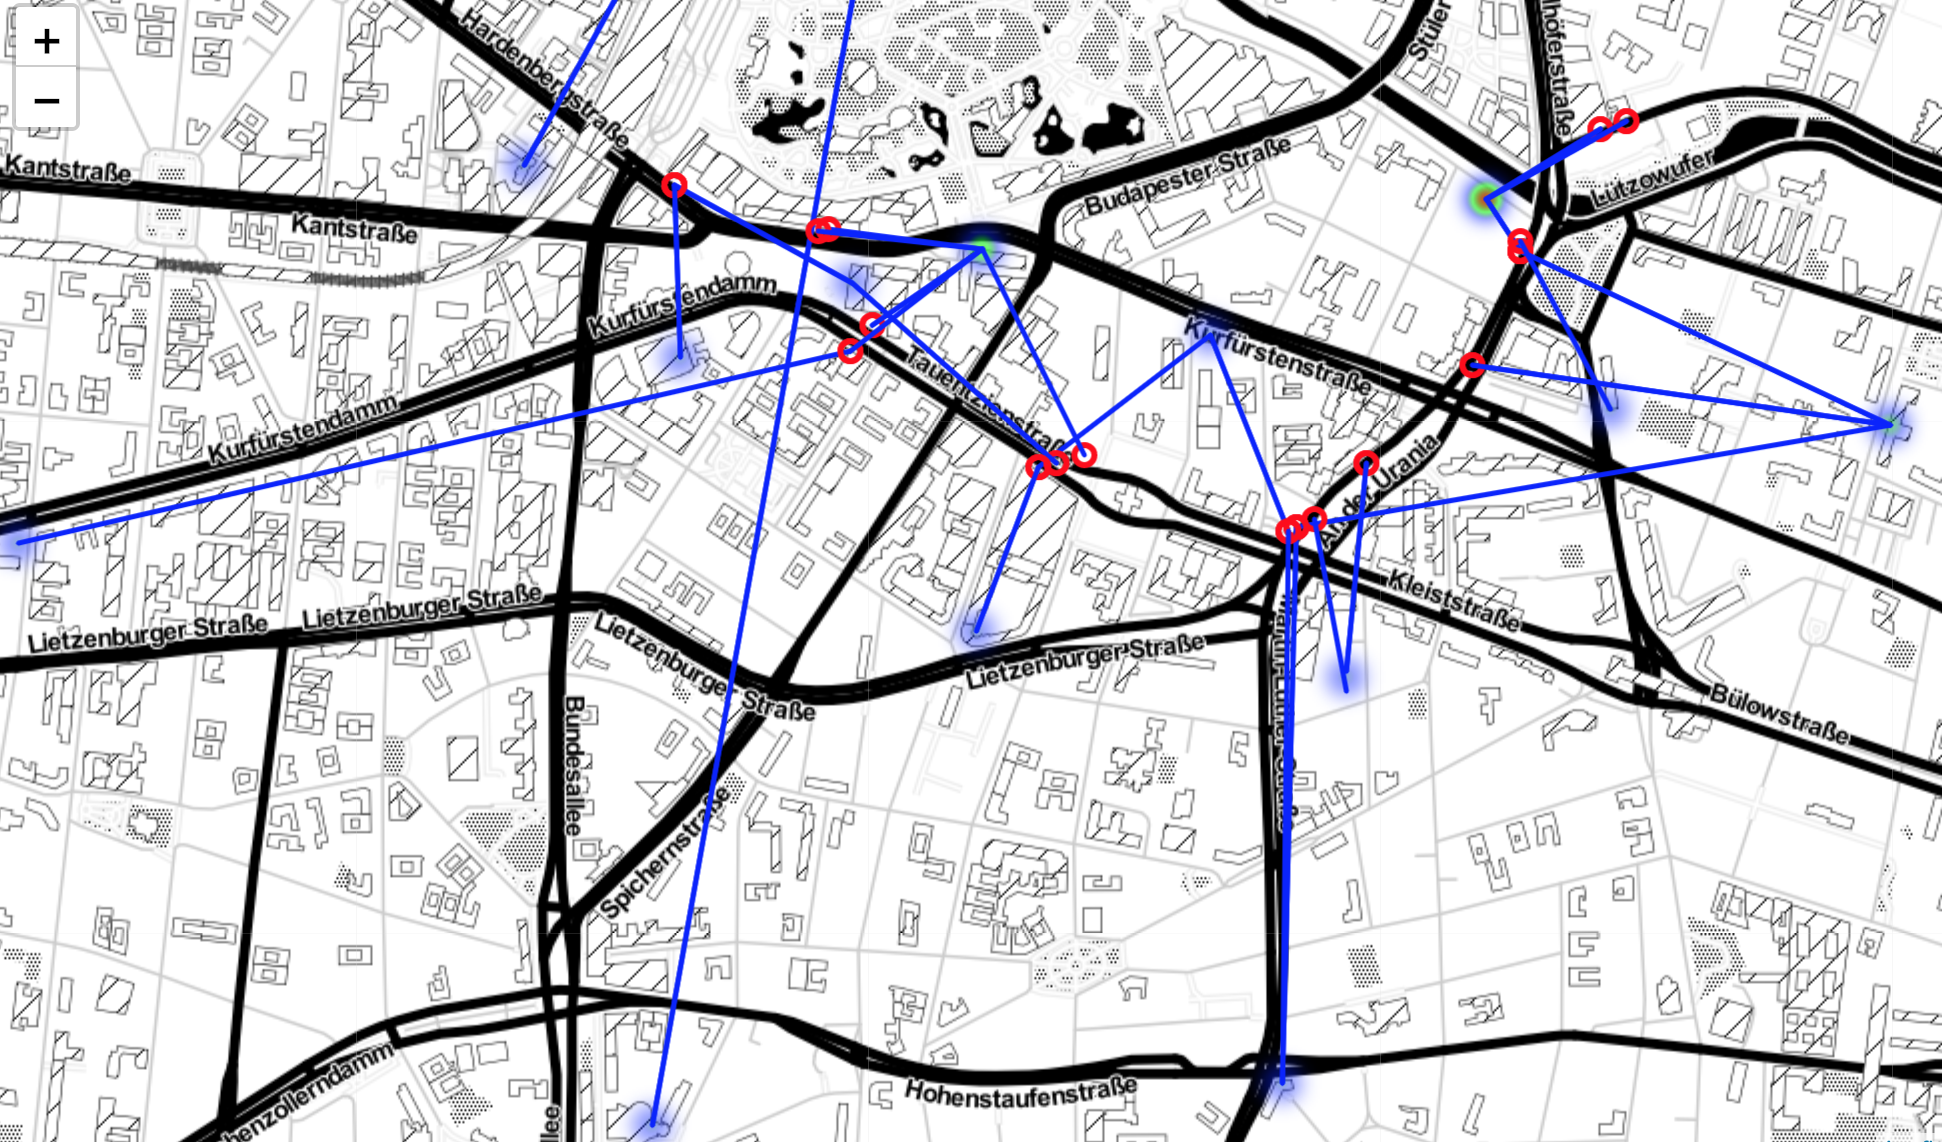
\includegraphics[width=0.5\textwidth]{images/localization_eval.png}
    \caption{Problem illustration}
    \label{fig:problem}
\end{figure}

In Figure\ref{fig:problem} and in the upcoming figures we use the following notation:
\begin{itemize}
    \item red circle - GPS observation,
    \item heat map - CDR location, i.e. location of assigned cell to CDR event,
    \item blue line - distance of GPS and CDR location.
\end{itemize}

\newdef{definition}{Definition}
\begin{definition}
A point $P(x,y)$ can be defined as a pair of latitude $y$ and longitude $x$ values representing a geographical location.
\end{definition}

A trajectory reflects the motion history of a moving object. In practice trajectory is not continuous due to the limited sampling capability, therefore one reasonable approach is to consider trajectories as a sequence of points.

\begin{definition}
A trajectory $T$ with length $n$ is defined as a time-stamped sequence of its consecutive points: \[T={(t,P_{1}), (t,P_{2}), .. (t,P_{n}}), T \in M\]
where $M$ is the set of possible trajectories.
\end{definition}

Evaluating cellular network event based customer positioning boils down to defining and calculating a distance or (dis)similarity measure between point based trajectories.

In this paper we do not attempt to reconstruct trajectories from CDR data considering the road network of Berlin. Instead we consider the sequence of positioned mobile network events together with the GPS trajectories and we try to determine the distance of the two trajectories based on the distances of individual pairs of points.

We use the distance definition of Deza et al. (\cite{encyclopedia}) in \cite{distance-def}. 

\begin{definition}
Let $\mathcal{T}$ be a set of trajectories. A function $d :\mathcal{T} \times \mathcal{T} \rightarrow \mathcal{R}$ is called a dissimilarity (distance) on $\mathcal{T}$ if for all $T_{1}, T_{2} \in \mathcal{T}$: 
\begin{itemize}
    \item $D(T_{1},T_{2}) \geqslant 0$
    \item $D(T_{1},T_{2}) = d(T_{2},T_{2})$
    \item $D(T_{1},T_{1}) = 0$
\end{itemize}
If all of these conditions are satisfied and $D(T_{1}, T_{2}) = 0 \Rightarrow  T_{1} = T_{2} $ is considered to be a symmetric. If
the triangle inequality is also satisfied, $D$ is a metric.
\end{definition}





